\documentclass[10pt,xcolor=x11names,dvipsnames,hyperref={colorlinks=false,breaklinks=true,bookmarks=true}]{beamer}
\usepackage{stylesheet}
%\usepackage{pgfpages}
%\setbeameroption{show notes on second screen}

\begin{document}

% TITLE, AUTHOR, DATE, INSTITUTE
\title[]{\textbf{Lower Bounds and Algorithms\\ in the\\ Linear Decision Tree Model\vspace{3mm}}}
\author[]{\large AURÉLIEN OOMS\\ADVISOR: PROF. JEAN CARDINAL\vspace{5mm}}
\institute[]{%
\footnotesize MÉMOIRE PRÉSENTÉ EN VUE DE L'OBTENTION\\
DU DIPLÔME DU MASTER EN SCIENCES INFORMATIQUES\\
ANNÉE ACADÉMIQUE 2014~-~2015\\[3mm]
\small UNIVERSITÉ LIBRE DE BRUXELLES}
\date{}

\begin{frame}
\titlepage{}
\end{frame}

\section{Introduction}
\begin{frame}\frametitle{\insertsection}\justifying
We focus on studying the complexity of problems and solving problems
in the linear decision tree model. In the model we use, solving a problem
amounts to retrieve information. We are allowed to retrieve information
through an oracle by means of questions that
can be answered ``yes'' or ``no''.\\[7mm]\pause
\bblue{\large Outline}
\begin{itemize}[label={\color{prussianblue}$\bullet$},itemsep=6pt]
\item Decision Tree Model\pause
\item Information-Theoretic Lower Bound\pause
\item Sorting under Partial Information\pause
\item \(k\)-linear Degeneracy Testing\pause
\item Application of Meiser's Algorithm
\end{itemize}
\end{frame}

\section{Decision Tree Model}
\begin{frame}\frametitle{\insertsection}\justifying
\begin{defn}[(Decision Tree Model)]
We are allowed to ask questions to an oracle \(\le\) that are answered
``yes'' or ``no''. Hence, each answer gives us at most
one additional bit of information.
Each question asked to the oracle costs us a single unit.
Every other operation can be carried out for free.
\end{defn}\pause
The goal of each of our analyses is to show that at least a certain
number of questions are required to be asked to solve a given problem, or
to provide an algorithm solving this problem using at most a certain number of
questions. Those two kinds of results are called lower bounds and upper bounds
respectively. A lower bound or an upper bound is in general expressed as
a function of the input size.
\end{frame}

\section{Information-Theoretic Lower Bound}
\begin{frame}\frametitle{\insertsection}\justifying
\begin{defn}[(\textsc{ITLB})]
The \emph{information-theoretic lower bound} (\textsc{ITLB}) of a problem
is the minimal depth of any
decision tree solving this problem. Generally speaking, the value of this lower
bound is the logarithm\footnote{Throughout this presentation, \(\log x\) denotes the binary logarithm of \(x\).}
in base \(2\) of the number of feasible solutions for this problem.
\end{defn}\pause
This lower bound is our goal to attain in terms of number of questions
when designing an efficient algorithm solving a problem. If \(\Gamma\) is the
set of feasible solutions of our problem, the \textsc{ITLB} only means
that we cannot do better than \(\ceil{\log(\Gamma)}\) questions, but it does not
necessarily mean that there exists an algorithm or a decision tree achieving
this bound in terms of complexity.
\end{frame}


\section{Sorting under Partial Information}
\begin{frame}\frametitle{\insertsection}\justifying
\begin{probl}[Sorting under Partial Information (\textsc{SUPI})]
Let \(\S = \enum{s_1 , \ldots , s_n}\) be a set
equipped with an unknown linear order. Given a subset of the relations \(s_i
\leq s_j\), determine the complete linear order by queries of the form
\(s_i \ask{\leq} s_j\).
\end{probl}\pause

\begin{ex}[(\textsc{SUPI})]
\parbox[b][3cm][t]{.45\textwidth}{
\psset{unit=.95cm}
\begin{pspicture}(-0.5,2.32)(3.5,0.82)
{\psset{linewidth=1.0pt}
\begin{footnotesize}
\only<2->{\psset{labelsep=0pt}
\uput{3pt}[225](0.5,0.5){\(c\)}
\uput{0.2pt}[315](1.,0.5){\(d\)}
\uput{2.5pt}[135](0.5,1.){\(a\)}
\uput{2.5pt}[45](1.,1.){\(b\)}
}
\end{footnotesize}
\only<2->{\psset{linecolor=black}
\psline(0.5,0.5)(0.5,1.)
\psline(0.5,0.5)(1.,1.)
\psline(1.,1.)(1.,0.5)
\psdots(0.5,0.5)
\psdots(1.,0.5)
\psdots(0.5,1.)
\psdots(1.,1.)
}
\only<3->{{\psset{linestyle=dotted}
\psline(0.5,1.)(1.,1.)
}}
\only<4->{
\psline{->}(1.5,.75)(1.75,.75)
}
\begin{footnotesize}
\only<4->{\psset{labelsep=0pt}
\uput{3pt}[225](2,0.25){\(c\)}
\uput{0.2pt}[315](2.5,0.25){\(d\)}
\uput{2.5pt}[135](2.25,1.25){\(a\)}
\uput{2.5pt}[135](2.25,0.75){\(b\)}
}
\end{footnotesize}
\only<4->{\psset{linecolor=black}
\psline(2.25,1.25)(2.25,0.75)
\psline(2.25,0.75)(2.,0.25)
\psline(2.25,0.75)(2.5,0.25)
\psdots(2.25,0.75)
\psdots(2.25,1.25)
\psdots(2.,0.25)
\psdots(2.5,0.25)
}
\only<5->{{\psset{linestyle=dotted}
\psline(2,.25)(2.5,.25)
}}
\only<6->{
\psline{->}(3.,.75)(3.25,.75)
}
\begin{footnotesize}
\only<6->{\psset{labelsep=0pt}
\uput{2.5pt}[135](3.75,0.5){\(c\)}
\uput{2.5pt}[135](3.75,0.0){\(d\)}
\uput{2.5pt}[135](3.75,1.5){\(a\)}
\uput{2.5pt}[135](3.75,1.0){\(b\)}
}
\end{footnotesize}
\only<6->{\psset{linecolor=black}
\psline(3.75,1.5)(3.75,1.0)
\psline(3.75,1.0)(3.75,0.5)
\psline(3.75,1.0)(3.75,0.0)
\psdots(3.75,1.0)
\psdots(3.75,1.5)
\psdots(3.75,0.5)
\psdots(3.75,0.0)
}
}
\end{pspicture}
}\hspace{3mm}\parbox[b][3cm][c]{.55\textwidth}{\centering
\only<2>{A partially ordered set for which we want to find a linear extension.}
\only<3>{We query the oracle with \(a \ask{\le} b\).}
\only<4>{The answer is ``yes''.}
\only<5>{We query the oracle with \(d \ask{\le} c\).}
\only<6>{The answer is ``no''.}}
\end{ex}
\end{frame}

\begin{frame}\frametitle{\insertsection}\justifying
\begin{thm}[(\textsc{ITLB} of \textsc{SUPI})]
Given a poset \(\P\), computing a linear extension of \(\P\) requires at
least \(\log e(\P)\) queries.
\end{thm}\pause
\proof
A decision tree that computes a linear extension of \(\P\) has \(e(\P)\)
leaves. The height of this tree is at least \(\log e(\P)\).
\endproof\pause

\parbox[b][][c]{1\textwidth}{\centering
\psset{unit=.75cm}
\begin{pspicture}(-2.,-3.5)(5.5,3.5)
\only<3->{\psset{fillstyle=solid,fillcolor=darkgray!3!white,linecolor=darkgray,linewidth=1.35pt}
\rput{-0.916}(1.646,-0.026){\psellipse(0,0)(3.526,3.118)}}
\only<4>{\psset{fillstyle=solid,fillcolor=MediumOrchid2!18!white,linecolor=MediumOrchid2,linewidth=1.35pt}
\rput{40.892}(2.029,-1.02){\psellipse(0,0)(1.622,1.332)}}
\begin{small}
\only<3->{\uput[45](3.726,2.418){\color{darkgray}\(n!\)}}
\only<4>{\uput[45](3.448,-0.275){\color{MediumOrchid2}\(e(\P\))}}
\end{small}
\end{pspicture}}
\end{frame}

\section{\(k\)-linear Degeneracy Testing}
\begin{frame}\frametitle{\insertsection}\justifying
\begin{probl}[\(k\)-linear Degeneracy Testing (\(k\)-\textsf{LDT})]
Given a set \(\S \subset \R\), \(\card{\S} = n\), and \(k+1\) real
coefficients \(\alpha_0, \alpha_1, \ldots, \alpha_k \in \R\), decide whether
there exists a \(k\)-tuple
\((s_1, \ldots, s_k)\), \(s_i \in \S\), such that
\(\alpha_0 + \sum_{i=1}^{k} \alpha_i s_i = 0\).
\end{probl}\pause
We consider a model where a comparison can be made
between more than two elements. A ``comparison'' between three elements
\(a\), \(b\), and \(c\) could be
for example \(2a - 3b + c \ask{\le} 0\). Decisions based on the result of such
a comparison depend on the sign of the expression \(2a - 3b + c\), that is, whether
this expression is less than, equal to or greater than \(0\).
In this model, we are only allowed to query for linear combinations of
input elements. This generic model is the \emph{linear decision tree
model}.
\end{frame}

\section{Application of Meiser's Algorithm}
\begin{frame}\frametitle{\insertsection}\justifying
\begin{probl}[Point location problem in an arrangement of hyperplanes]
Given a point $x \in \R^n$ and a set of hyperplanes $\H = \enum{ H_i
\st 1 \leq i \leq m }$ determine the position vector of $x$, $\pv(x) \in
\signset^n$, where $\pv_i(x) = \sigma, \sigma \in \signset$ iff $x \in
H_i^{\sigma}$. We define $H_i^{0}$, $H_i^{-}$ and $H_i^{+}$ to be
respectively $H_i$ itself, the half-space below $H_i$ and the half-space above
$H_i$.
\end{probl}\pause
We can convert any instance of the \(k\)-\textsf{LDT} problem into an
instance of the point location problem in an arrangement of hyperplanes.
By agreeing on an order of the elements of \(\S\) (for example, the total order on
the real numbers) we can associate a unique \(n\)-tuple to each set \(\S\),
and thus a unique point \(x\) in \(\R^n\) for each \(\S\).
For each \(k\)-tuple \((s_1, \ldots, s_k)\) we need to find whether
\(\alpha_0 + \alpha_1 s_1 + \dots + \alpha_k s_k\)
is equal to zero. In our new representation of the problem this
boils down to deciding whether our point \(x\) lies on the hyperplane of
equation \(\alpha_0 + \alpha_1 s_1 + \dots + \alpha_k s_k = 0\). There are \(n^k\) such
hyperplanes, and to solve the problem
we have to decide whether \(x\) lies on one of them.
\end{frame}


\begin{frame}\frametitle{\insertsection}\justifying
\begin{thm}[(Clarkson)]\label{thm:meiser:clarkson}
Given a set $\H$ of $m$ hyperplanes in $\R^n$ and $\epsilon$ with the
constraint that $0 < \epsilon < 1$, there exists a subset $\NH \subseteq \H$ of
size $\BigO{\enetsize}$ such that for every simplex $\simplex$ in $\R^n$, if the
number of hyperplanes of $\H$ intersecting $\simplex$ is strictly greater than
$\epsilon \card{\H}$ then at least one of them belongs to $\NH$.
\end{thm}\pause
\begin{overlayarea}{\textwidth}{0.4\textheight}
\only<2>{\begin{cor}
If we choose $\BigO{\enetsize}$ hyperplanes uniformly at
random from \(\H\) and denote this selection $\H^{*}$ then for
any simplex intersected by more than $\epsilon \card{\H}$ hyperplanes of $\H$
there is a high probability that at least one of them is contained in $\H^{*}$.
\end{cor}}
\only<3>{\begin{cor}
If we choose $\BigO{\enetsize}$ hyperplanes uniformly at
random from \(\H\) and denote this selection $\H^{*}$ and
if there is no hyperplane in $\H^{*}$ intersecting a given simplex, then, with
high probability, the number of hyperplanes of $\H$ intersecting the simplex
is less or equal to $\epsilon \card{\H}$.
\end{cor}}
\end{overlayarea}
\end{frame}

\begin{frame}\frametitle{\insertsection}\justifying
\begin{figure}
\begin{center}
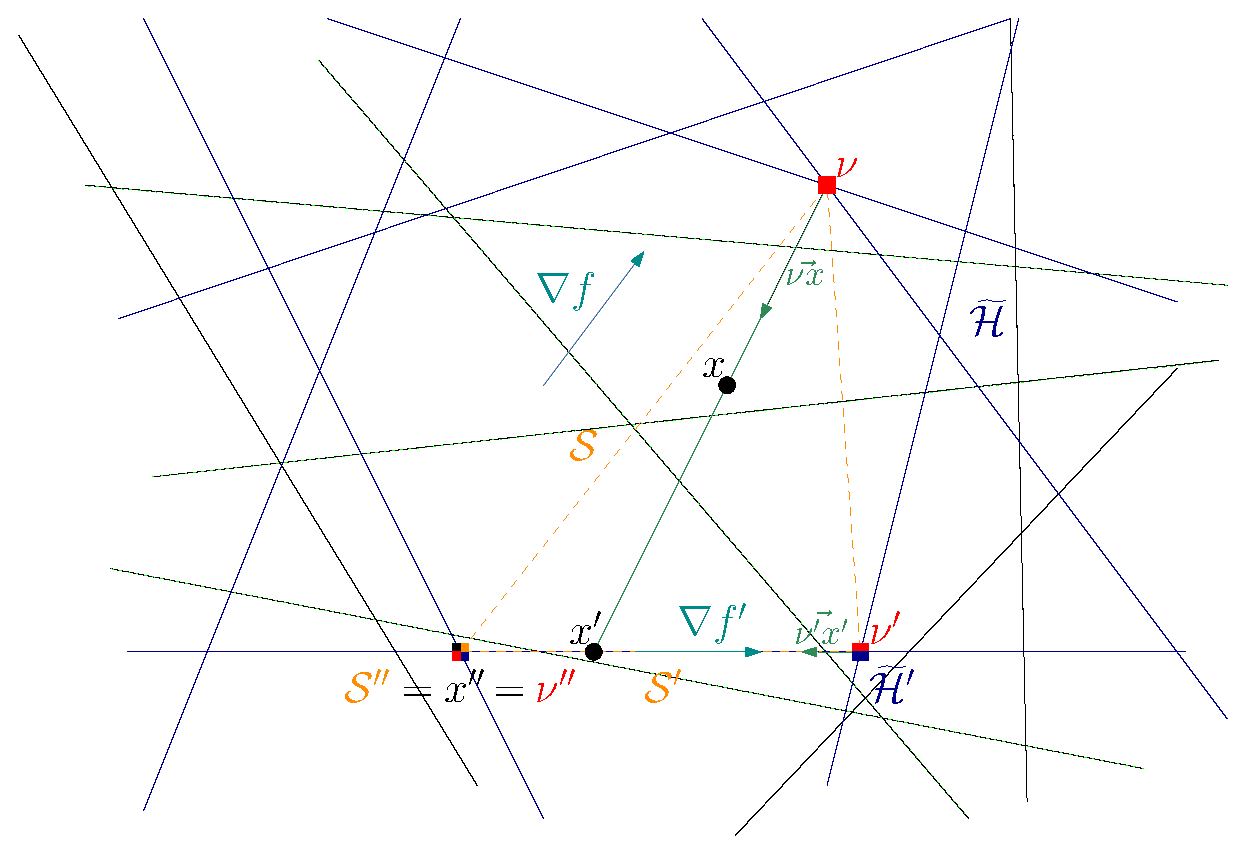
\includegraphics[trim=110 40 50 30,clip=true,height=0.6\textheight]{../report/fig/point-location/simplex.eps}
\caption{
A complete step of Meiser's algorithm. The blue lines are hyperplanes of the
set \(\widetilde{\H}\). The gradient of the objective function
chosen to find the first vertex of the simplex is \(\nabla f\). The green dotted lines are the
hyperplanes from \(\H \setminus \widetilde{\H}\) that meet \(\S\), those are
the only hyperplanes that are left to process after this step.
}
\end{center}
\end{figure}
\end{frame}

\begin{frame}\frametitle{\insertsection}\justifying
\begin{algo}[(Building \(\simplex\))]
\item[input] A point \(x\) and a set of hyperplanes \(\widetilde{\H}\) in
\(\R^n\).
\item[1.] Find a vertex $\nu$ of the cell containing $x$, $\nu$ is one of
the vertices of our simplex.
\item[2.] Compute $x'$, the projection of $x$ along $\vec{\nu x}$ on the
boundary of \(\cell\).
\item[3.] Let \(H_{\theta}\) denote the hyperplane in \(\widetilde{\H}\)
containing \(x'\). Compute \(\widetilde{\H}'\) as the intersection of all
hyperplanes of \(\widetilde{\H} \setminus \enum{H_{\theta}}\) with
\(H_{\theta}\).
\item[4.] Induction on \(x'\) and \(\widetilde{\H}'\) in $\R^{n-1}$, store result in \(\simplex'\).
\item[5.] Return \(\simplex\), the convex hull of \(\simplex' \cup \enum{\nu}\).
\end{algo}\pause
We choose \(\card{\Ht} = \BigO{\enetsize}\) and compute  the cell $\cell$ of the
arrangement $\arrangement(\Ht)$ containing $x$, then we refine the cell around
point $x$. We do so by computing a simplex $\simplex$ inscribed in $\cell$ and
containing \(x\). Then we discard hyperplanes that do not meet this simplex.
\end{frame}

\begin{frame}\frametitle{\insertsection}\justifying
\begin{algo}[(Meiser's algorithm)]
\item[input] $x \in \R^n$, the point to be located.
\item[1.] Compute the position of $\BigO{n^2 \log^2 n}$ hyperplanes relatively to
$x$, effectively computing cell $\cell$ containing $x$.
\item[2.] Recursively build simplex $\simplex$ containing $x$ and inscribed in
$\cell$.
\item[3.] For any hyperplane $H_i$ not meeting the simplex, deduce $\pv_i(x)$.
\item[4.] Discard all hyperplanes that do not meet the inside of the
simplex.
\item[5.] Recurse on hyperplanes that are left.
\end{algo}\pause

Since the complexity of step \step{1} is \BigO{n^2 \log^2 n}, the complexity of step
\step{2} is \BigO{n^3 \log^2 n}, the complexity of steps \step{3} and \step{4}
is \(0\),
and the induction depth is $\BigO{\log m}$, the total complexity of this algorithm
is \BigO{n^3 \log^2 n \log m}. For our \(k\)-\textsf{LDT} problem, \(m = n^k\),
and thus the complexity is \BigO{k n^3 \log^3 n}. Note that the overall
complexity in the Random Access Machine model is polynomial.

\end{frame}
\end{document}
